\documentclass[12pt, a4paper, oneside]{ctexbook}
\usepackage{amsmath, amsthm, amssymb, bm, graphicx, hyperref, mathrsfs, float, subfigure, svg}

\title{{\Huge{\textbf{Chapter1 神经元和数学方法}}}}
\author{黄志权}
\date{\today}
\linespread{1.5}
\newtheorem{theorem}{定理}[section]
\newtheorem{definition}[theorem]{定义}
\newtheorem{lemma}[theorem]{引理}
\newtheorem{corollary}[theorem]{推论}
\newtheorem{example}[theorem]{例}
\newtheorem{proposition}[theorem]{命题}
\CTEXsetup[format={\Large\bfseries}]{section}

\begin{document}

\maketitle

\pagenumbering{roman}
\setcounter{page}{1}

\newpage
\pagenumbering{Roman}
\setcounter{page}{1}
\tableofcontents
\newpage
\setcounter{page}{1}
\pagenumbering{arabic}

\chapter{IF模型(Integrate-and-fire models)}
神经元的动力模型可以被简化为:树突接收若干的脉冲信号,并积累到细胞膜上,致使细胞膜电压改变,从而产生动作电位。LF模型则是将动作电位描述成事件的模型。它由两个部分组成:1、描述膜电压$u(t)$演变的线性微分方程;2、描述spike的发射机制。

\section{膜电压$u(t)$演变的线性微分方程推导}
对于神经元细胞,我们可以将其想象为如下的RC电路。细胞膜就像是一个与电阻并联的电容器,而电阻连接着一个电压为$u_{rest}$电池。当没有外界输入时,膜电压$u(t)$为初始值$u_{rest}$;当有外界脉冲输入时,相当于给电容提供电流为$I(t)$的充电,从而改变模电压$u(t)$。//PS:这个电阻也被称为漏电阻。由于在没有外界输入时,膜上电荷会逐渐穿过细胞膜泄露出去,让膜电压回归$u_{rest}$,因此引入一个漏电阻来模拟这种现象。

\begin{figure}[H]
    \centering
    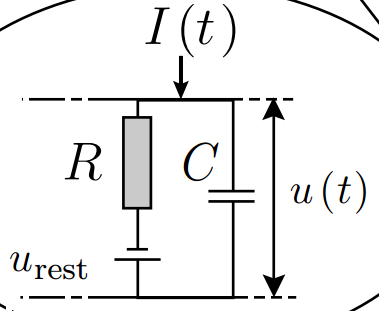
\includegraphics[width=0.3\textwidth]{细胞膜等效电路.png}
    \caption{细胞膜等效电路}
\end{figure} 

考虑$I(t)$不为零的情况,即有外界输入时,来分析膜电压的变化。首先总电流由并联电路支电流和组成$I(t)=I_r+I_C$。即:

\begin{equation}
I(t)=\frac{u(t)-u_{rest}}{R}+C\frac{du(t)}{dt}    
\end{equation}

模仿电路分析,定义膜时间常数(membrane time constant)$\tau _m=RC$。从而可以得到$u(t)$的线性微分方程:

\begin{equation}
    \tau _m\frac{du(t)}{dt}= -[u(t)-u_{rest}] + RI(t)
\end{equation}

上式在电路分析中称为RC电路响应方程,在神经科学领域称为无源膜方程(equation of a passive membrane)。这个方程的解分为两个部分。即输入脉冲的充电过程(零状态响应),和没有输入脉冲,电压泄露到$u_{rest}$的过程(零状态响应)。首先是输入脉冲的充电过程(零状态响应),我们假设输入电流脉冲是一个幅值为$I_{max}$的方波,则其方程如下:

\begin{equation}
    u(t)=u_{rest}+I_{max}R(1-e^{-\frac{t}{\tau}})
    \label{零状态响应}
\end{equation}

\begin{figure}[H]
    \centering
    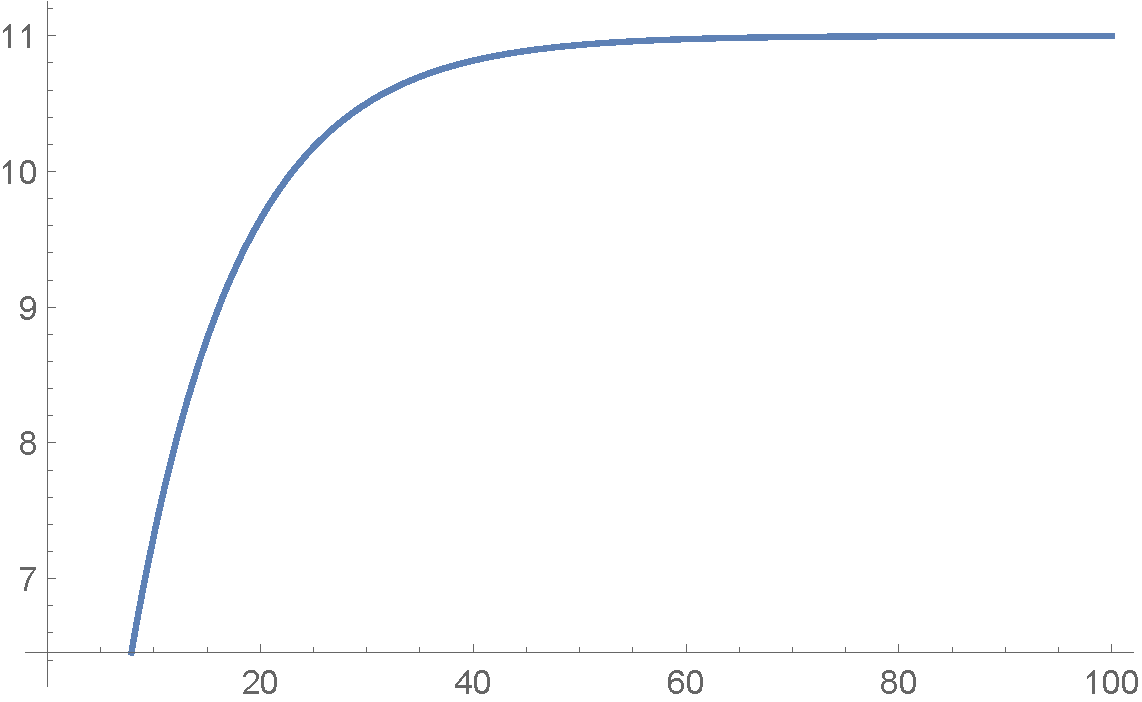
\includegraphics[width=0.5\textwidth]{脉冲充电图.pdf}
    \caption{脉冲充电图}
\end{figure} 

然后是电压泄露到$u_{rest}$的过程(零状态响应):

\begin{equation}
    u(t)=u_{rest}+I_{max}Re^{-\frac{t}{\tau}}
    \label{零输入响应}
\end{equation}

\begin{figure}[H]
    \centering
    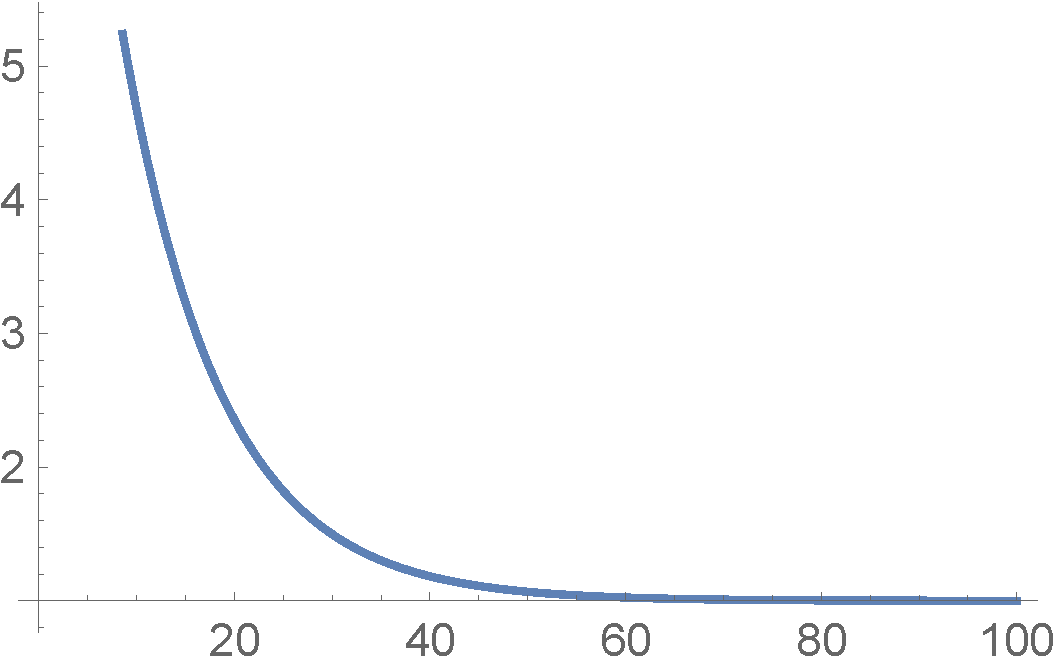
\includegraphics[width=0.5\textwidth]{脉冲放电图.pdf}
    \caption{脉冲放电图}
\end{figure} 

从而,当没有外部脉冲输入的情况下,膜电压会以指数形式衰减到$u_{rest}$。其衰减时间系数$\tau m$一般为10ms,与一般持续1ms的尖峰脉冲相比长了很多。

接下来,考虑输入电流I(t)为一个短的脉冲。因为是有脉冲输入,因此对应的是公式\ref*{零状态响应}。

\end{document}